\label{sec:intro}
As has already happened in the image domain, the wide availability of 3D models brings with it the need to associate semantic information with the 3D data. In this work we focus on the problem of annotating 3D models represented by 2D meshes with part information. Understanding of the parts of an object (e.g., the back, seat and legs of a chair) is essential to its geometric structure, to its style, and to its function. % Part structure is also often correlated with appearance and material information (e.g., object textures). 
There has been significant recent progress~\cite{Yi16} in the large scale part annotation of 3D models (e.g., for a subset of the ShapeNet~\cite{shapenet2015} models) -- our aim here is to leverage this rich data set so as to infer parts of new 3D object models. Our techniques can also be used to infer keypoints and other substructures within 3D models.

It is not straightforward to apply traditional deep learning approaches to 3D models because a mesh representation can be combinatorially irregular and does not permit the optimizations exploited by convolutional approaches, such as weight sharing, which depend on regular grid structures. In this paper we take a functional approach to represent information about shapes, starting with the observation that a shape part is itself nothing but a 0-1 indicator function defined on the shape. 

Our basic problem is to learn functions on shapes. We start with example functions provided on a given shape collection in the training set and build a neural net that can infer the same function when given a new 3D model. This suggests the use of a spectral formulation, based on a dual graph representing the shape, yielding bases for a function space built over the mesh.  % Although we can use the eigenfunctions of mesh laplacian for this purpose, in this work we choose to replace each shape by a set of sample points and then use the nearest-neighbor graph laplacian of this point cloud to encode functions on the point cloud (including parts). The point sample approach (based on furthest point sampling) makes representations more independent of the particularities of the mesh and also can be used directly on point cloud representations of 3D geometry.

\begin{figure}
    \centering
    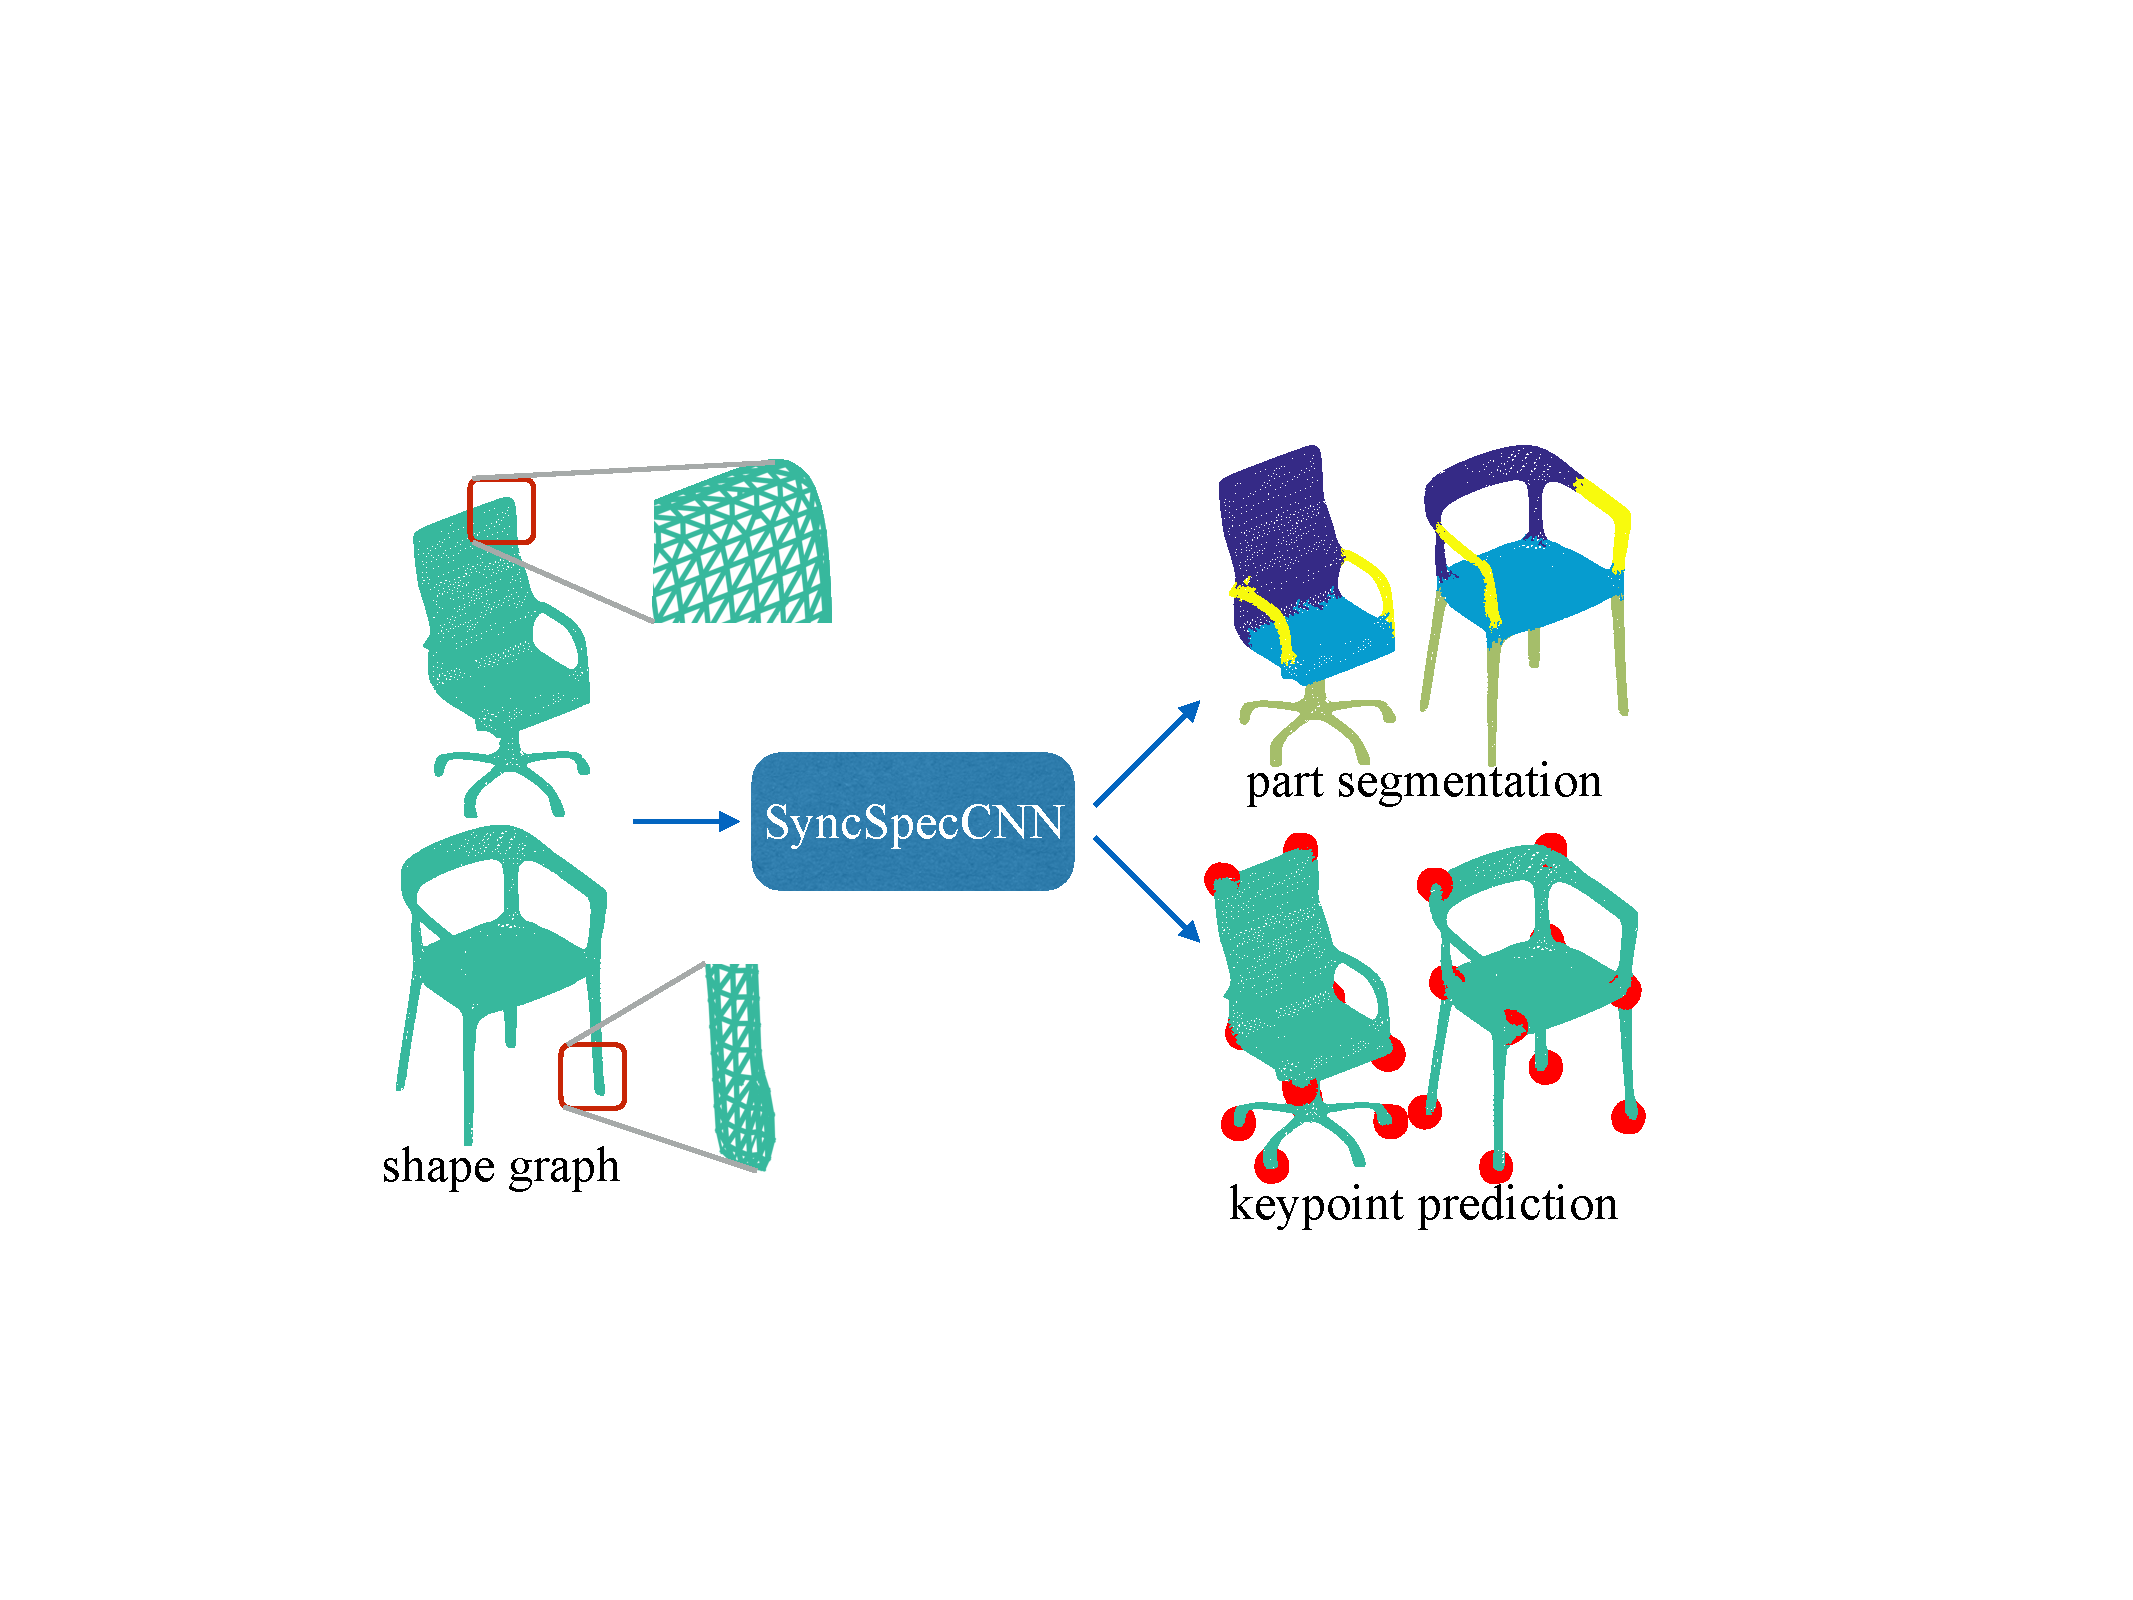
\includegraphics[width=0.4\textwidth]{./fig/teaser3.pdf}
    \caption{Our SyncSpecCNN takes a shape graph equipped with vertex functions (i.e. spatial coordinate function) as input and predicts a per-vertex label. The framework is general and not limited to a specific type of output. We show 3D part segmentation and 3D keypoint prediction as example outputs here. }
    \label{fig:teaser}
    \vspace{-0.3cm}

\end{figure}

With this graph representation we face multiple challenges in building a convolutional neural architecture. One is how to share coefficients and conduct multiscale analysis in different parts of the graph for a single shape. Another is how to share information across related but different shapes that may be represented by very different graphs. We introduce a novel architecture, the Synchronized Spectral CNN (SyncSpecCNN) to address these issues. 

The basic architecture of our neural network is similar to the fully convolutional segmentation network of~\cite{long2015fully}, namely, we repeat the operation of convolving a vertex function by kernels and applying a non-linear transformation. However, our network combines processing in the primal and dual (spectral) domains. %, including aligning different shapes in the spectral domain using functional maps, in the style of a spectral transformer network. 
We deal with the problem of weight sharing among convolution kernels at different scales in the primal domain by performing the convolutions in the spectral domain, where they become just pointwise multiplications by the kernel duals. %As is well-known, multiscale kernels are important for convolutional architectures in order to capture a wide context --- in our setting, these kernel duals become modulated exponential windows that shrink as the primal kernels expand. 
Our key building block consists of passing to the dual, performing a pointwise multiplication and then returning to the primal representation in order to perform an appropriate non-linear step (such operations are not easily dualized).

The issue of information sharing across shapes is more challenging.  Since different shapes give rise to different nearest neighbor graphs on their point clouds, the eigenbases we get for the graph laplacians are not directly comparable. We synchronize all these laplacians by applying a functional map in the spectral domain to align them to a common canonical space. %Synchronization is most important for the low frequency eigenfunctions, as these are used to encode the duals of large kernels in the primal domain. 
The aligning functional maps succeed in encoding all the dual information on a common set of basis functions where global learning takes place. An initial version of the aligning maps is computed directly from the geometry and then is further refined during training, in the style of a data-dependent spatial transformer network. %Another such alignment map is also used in a later stage of the network.

% When the set of shapes to be considered is very diverse, (dual) alignment to a single prototype may cast unwanted distortions. For this reason we allow encodings to multiple prototypes and let the deep net use all of them, disentangling where the reliable invocation is to be found.

We have tested our SyncSpecCNN on various tasks including 3D shape part segmentation and 3D keypoint prediction. We achieve state-of-the-art performance on all these tasks.

Key contributions of our approach are as follows:% ... [say that this is a general framework for learning general functions on shapes, not just parts or keypoints
\bitem
    \item We are the first to target at non-isometric shapes in the family of spectral CNNs.%, unlike existing spectral CNNs that mostly target at near-isometric shapes such as human bodies.%, our SyncSpecCNN can work well for generic shapes with large topological and geometrical variation. %, such as furnitures that have highly different manufacturing structure.
    % \item To allow weight sharing across different non-isometric shapes, we synchronize the spectral domain of each shape to a canonical domain, achieved by learning a Spectral Transformer Network.
    \item To allow weight sharing across different non-isometric shapes, we learn a Spectral Transformer Network.
    % \item We introduce a spectral parameterization of dilated convolutional kernels, allowing the construction of kernels at large scales with parsimonious parameters. % This parsimonious parameterization of kernels allows us to capture features at multi-scales without incurring signicant overfitting. 
    \item We introduce an effective spectral multiscale kernel construction scheme. % This parsimonious parameterization of kernels allows us to capture features at multi-scales without incurring signicant overfitting. 
% \item a deep learning framework that combines both intrinsic and extrinsic geometric properties of input 3D shape
\eitem



\iffalse
\todo{
  some dumps of thoughts:
  \begin{itemize}
  \item{A good 3D representation should be flexible to encode both intrinsic and extrinsic property of the underlying 3D shape. Voxel, multiview images treat non-euclidean domain as euclidean domains and might lose details about the object and break the topological structure. Mesh representation, which not only considers vertex positions of a 3D shape but also encodes connectivity relationship among vertices, serves this purpose well.}
  \item{Existing deep learning framework which consumes mesh representation mostly focuses on near isometric shapes and designs localized convolutional kernels to aggregate information. The key issue here is each mesh being an independent non-euclidean domain makes it hard to share parameters and generalize.} \item{We propose a way to learn to align different non-euclidean domains } \end{itemize}
}
\fi
